\documentclass[format=acmsmall, review=false, screen=true]{acmart}
\settopmatter{printacmref=false} % Removes citation information below abstract
\renewcommand\footnotetextcopyrightpermission[1]{} % removes footnote with conference information in first column
\pagestyle{plain} % removes running headers
\acmYear{2018}
\acmMonth{7}

\usepackage[utf8]{inputenc}
\usepackage{microtype}
\usepackage{amsmath}
\usepackage[procnames]{listings}
\usepackage{amsmath}
\usepackage{float}
\usepackage{wrapfig}
\usepackage{subcaption}
\usepackage{dirtytalk}
\usepackage{color}

\lstset{
  basicstyle=\ttfamily,
  columns=fullflexible,
  frame=single,
  breaklines=true,
  postbreak=\mbox{\textcolor{red}{$\hookrightarrow$}\space},
  aboveskip=10pt,
  belowskip=5pt,
  tabsize=2
}


\setlength{\textfloatsep}{15pt}
\setlength{\abovecaptionskip}{6pt}
\setlength{\belowcaptionskip}{6pt}

\author{Richard Banyi}
\affiliation{%
  \institution{IT University of Copenhagen}
  \streetaddress{Rued Langgaards Vej 7}
  \city{Copenhagen}
  \postcode{2300}
  \country{Denmark}
}

\email{riba@itu.dk}

\author{David Kadish}
\affiliation{%
  \institution{Supervisor}
}
\affiliation{%
  \institution{IT University of Copenhagen}
}
\affiliation{%
  \institution{Robotics, Evolution, and Art Lab}
}
\email{davk@itu.dk}

\author{Andres Faina}
\affiliation{%
  \institution{Supervisor}
}
\affiliation{%
  \institution{IT University of Copenhagen}
  \streetaddress{Rued Langgaards Vej 7}
  \city{Copenhagen}
  \postcode{2300}
  \country{Denmark}
}
\affiliation{%
  \institution{Robotics, Evolution, and Art Lab}
}
\email{anfv@itu.dk}


\title{\textsc{Thesis Preparation }}
\subtitle{\textsc{IT University of Copenhagen, Autumn 2018}}
\acmDOI{}
\begin{document}


\begin{abstract}

In machine learning field, particularly neuroevolution, evolved behaviors, that consists of distinctly different behaviors  are generally referred to as multimodal behavior. Recent work focused on developing various multi-objective evolutionary algorithms to solve multi-objective problems that are not explicitly defined as multi-objective problems. Because multimodal problems, are often too difficult to solve directly, some works exploits the combination of all possible subtask that can be optimized simultaneously on multiple subtask in order to solve the overall problem. These works often present different approaches on the same problem. Common for the projects is that they evolve the controllers using various evolutionary and neuroevolution techniques Additionally, the neural networks are combined with multi-objective optimization algorithms in order to focus on the desired objective of a given behavior. How to learn multimodal behaviors remains an interesting and difficult challenge. Taking on these challenges, this thesis aims to develop methods precisely to discover multimodal behaviors. While much of the recent projects involved optimizations in simulations, the thesis takes a further step and focus on evolving controllers using physical robot in real world test environment. Although there are many challenges to overcome in this domain, the primary motivation is to transfer from simulation to real world and show how evolution can act on real robot that has been less explored in the research area. Another novel element of the thesis, is that the reality-based optimization will involve mixed reality system. This will potentially enrich the environment and visualization moreover yield more modalities. This could prove to be useful to create various behaviors. The thesis builds on pre-existing neuroevolution algorithms and hardware components, which have been modified accordingly to the experiments. The system consists of several components, such as computer vision, to keep track about the environment and to provide fitness measurements used in fitness calculation. Furthermore, the system includes a robot on which the entire evolutionary process is performed. The system will be evaluated through series of tests that addresses the ability to evolve multimodal behavior for a single robot.

\end{abstract}

\maketitle

\section{Introduction}

Intelligent agents are defined as entities that carry out some set of operations on behalf of a user or a program with some degree of independence or autonomy, and in so doing, employ some knowledge or representation of the user's goals or desires. Such goals may involve variety of tasks to be solved. Solving diverse set of tasks requires the ability to exhibit multiple different behaviors. In machine learning field, behavior, is generally referred to as \emph{multimodal behavior} \footnote{\url{http://nn.cs.utexas.edu/?li:alife14}}. For example a harvesting robot have to behave differently depending whether it is harvesting tomatoes, strawberries \footnote{\url{http://www.dogtoothtech.com/}}, or searching for a dock to charge. In real world situation a self-driving vehicle has to be able to adapt to different environments, driving on the highway or on the country side requires different behavioral capabilities. All the mentioned tasks, whether harvesting or driving display similar or even dissimilar behaviors. Therefore, it is legitimate to say that intelligent agents must exhibit multimodal behaviors with respect to the changing environment.

The main challenges within these domains depends how to decouple the complex task into subtasks. How to accurately define the right behaviors? How to arbitrate between different behaviors? A behavior may be interrupted, by other behavior. Sometimes behavioral policies are human defined, other times are learned. Thus, it is difficult to build intelligent agents with multimodal behaviors. Recent work focused on developing multi-objective evolutionary algorithms (MOEA) \footnote{\url{https://brage.bibsys.no/xmlui/handle/11250/253596}} to solve multi-objective problems that are not explicitly defined as multi-objective. The algorithm attempts to define different ways to measure objectives and use ensembles to combine individual policies on the pareto front into a single controller. Another project\footnote{\url{https://arxiv.org/abs/1807.03392}} exploits the combination of all possible subtask that can optimize simultaneously on multiple subtask. 

These works offer different approaches on the same problem. Common for the projects is that they evolve the controllers using various evolutionary and neuroevolution techniques Additionally, the neural networks are combined with multi-objective optimization algorithms in order to focus on the desired objective of a given behavior.

How to learn multimodal behaviors is an interesting and difficult challenge. Taking on these challenges, this thesis aims to develop methods precisely to discover multimodal behavior. While the aforementioned projects involved optimizations in simulations, the thesis takes a further step and focus on evolving controllers using physical robot in real world test environment. Although there are many challenges to overcome in this domain, the primary motivation is to transfer from simulation to real world and show how evolution can act on real robot that has been less explored in the research area. Another novel element of the thesis, is that the reality-based optimization will involve mixed reality system. This will potentially enrich the environment and visualization moreover yield more modalities. This could prove to be useful to create various behaviors.


The thesis builds on pre-existing neuroevolution algorithms and hardware components.

\section{Related Work}

Learning multimodal behaviors can be diffult to solve directly. Many papers suggest to decouple the complex task into smaller related tasks. Rather than learning the complex task at once they focus on learning smaller related task first. The tasks are than combined and adjusted to form a more complex task. Therefore the smaller tasks represents crucial \emph{stepping stones} towards solving the complete task. The challenge is how to properly decouple the complex task into many subtask and in which order these subtask should interlieve to effectively form a more sophisticated behavior.

Joost Huizinga and Jeff Clune gave a good example \ref{fig:jumping_running} how these challenges can emerge in robot training task, which has to be able to learn both to run and jump. In their hypothetical example their argue, that running is much easier to learn than jumping, but learning to jump well first is an important stepping stone in order to become excelend in both tasks. Therefore individuals who are better at running, are more favorable than individuals that are average at jumping, and those individuals who are good at jumping are not selected in the future generations. An important stepping stone is lost during evolution. 

\begin{figure}[H]
  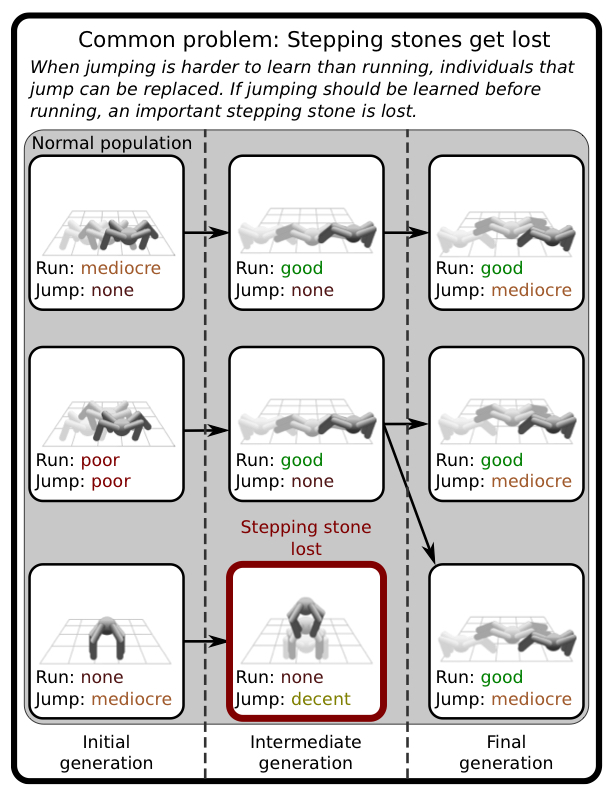
\includegraphics[width=0.46\linewidth]{img/jumping_running.JPEG}
  \caption{\label{fig:jumping_running}Stepping stones get lost}
\end{figure}

Joost Huizinga and Jeff Clune designed \emph{Combinatorial Multi-Objective Evolutionary Algorithm (CMOEA)} which is able to preserve the stepping stones of multimodal problems. The algorithm divides the population into bins, every bin is a combination of subtasks. Each set of subtasks has its own fitness function. The population is competing within bins, which helps to preserve important stepping stones to solve the overall problem. They have succesfully evolved a controller on a multimodal robotics problem with six subtaks.

The six tasks \emph{Forward, Backward, Turn-left, Turn-right, Jump, Crouch} needed to be learned by the robot. \emph{CMOEA} starts by generating a random number of individuals and adding copy of each individual to every bin. Selection is performed within each bin, with respect to the subtask associated with that bin. Each generation the algorithm selects a number of parents randomly across all bins. Each selected parents produce only one child by applying mutation (no crossver is applied) and is copied to every bin, afterwards selection is applied within each bin. The survivor selection method is applied by \emph{NSGA-II} with performance on the task associated with the given bin as one objective and \emph{behavioral diversity}\footnote{\url{https://www.researchgate.net/publication/51568478_Encouraging_Behavioral_Diversity_in_Evolutionary_Robotics_An_Empirical_Study}} as the other objective. Behavioral diversity ensure that individuals within each bin solves the same subtask in different ways. It's implemented by measuring the distance of some behavioral features between each individual in the same bin. All the controllers are neural networks evolved with \emph{NEAT} mutation operators without crossover, encoded with \emph{HyperNEAT}\footnote{\url{http://eplex.cs.ucf.edu/hyperNEATpage/}} encoding, which is extended with \emph{Multi-Spatial Substrate (MSS)}\footnote{\url{http://eplex.cs.ucf.edu/papers/pugh_gecco13_revised.pdf}} and a \emph{Link Expression Output}\footnote{\url{http://eplex.cs.ucf.edu/papers/verbancsics_gecco11.pdf}}.

\begin{figure}[H]
  \centering
  \begin{subfigure}[t]{0.55\textwidth}
    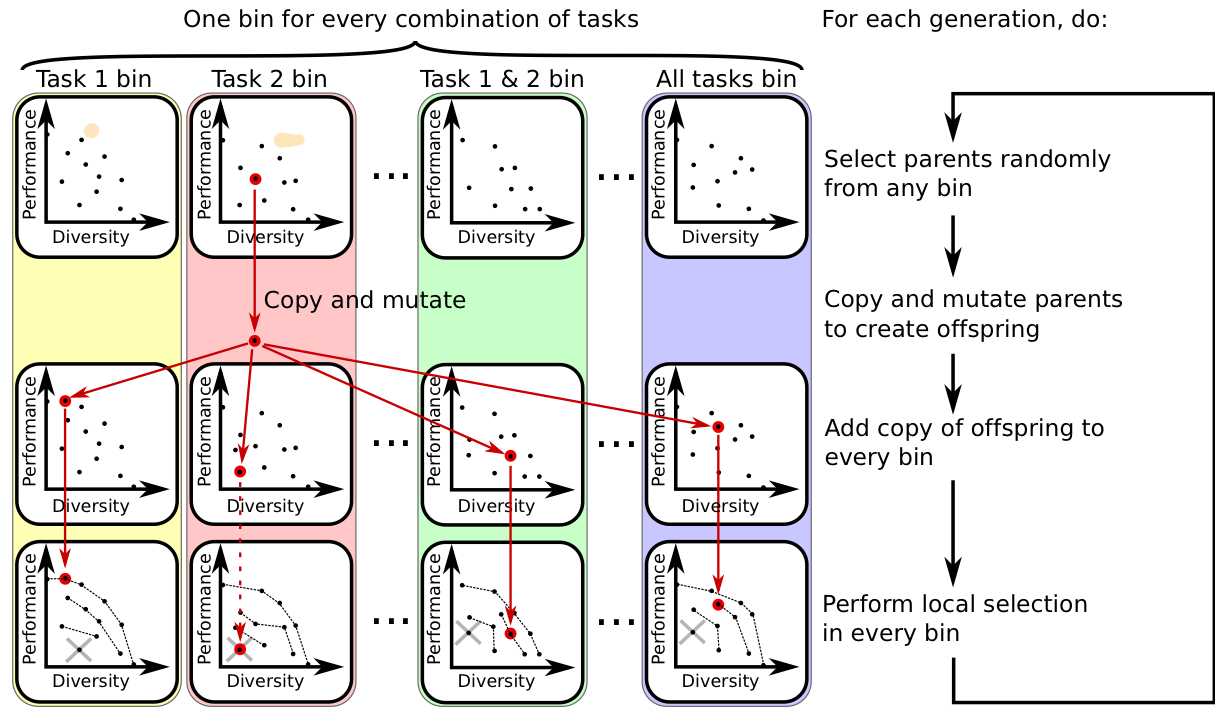
\includegraphics[width=\textwidth]{img/cmoea.JPEG}
    \caption{\label{fig:fronts}Overview of CMOEA}
  \end{subfigure}
  \hfill
  \begin{subfigure}[t]{0.43\textwidth}
    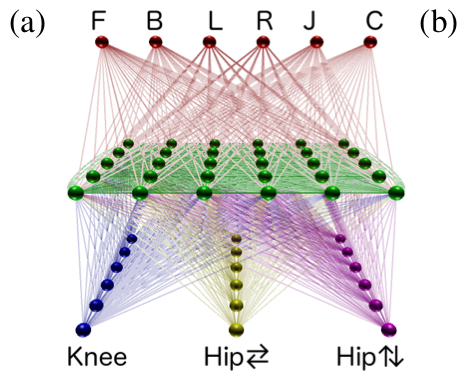
\includegraphics[width=\textwidth]{img/hyperneat.JPEG}
    \caption{\label{fig:endings}The spatial network layout, MSS planes.}
  \end{subfigure}
\end{figure}

In contrast to previous form of neuroevolution techniques with multi-objective optimization algorithms encouraging multimodal behaviors Stanley, Bryant and Miikkulaine presented an experiment named \emph{The Dangerous Foraging Domain}\footnote{\url{http://nn.cs.utexas.edu/downloads/papers/stanley.cec03.pdf}} which does not explicitly focus on developing multimodal behavior, however they produced agents that could potentially exhibit multimodal behavior. The experiment models a natural foraging environment. Where an agent enters a new region, some food may be edible or poisonous, or edible food could turn into poisonous one. The agent can't tell whether the food is edible without trying it first. Thus after the robot consume a piece of food has to decide whether it should continue foraging or a should avoid all food. The challenge in constructing such a networks is by the fact that in has to evolve policies for foraging of both safe and poisonous food, including the ability of abandoning policy when it encounter poison. The neural networks only received a pain and pleasure signal. The experiments where designed to test whether adaptive synapses are necessary for adaption. According to their results, the networks using recurrent connections performed well, since the recurrent connection on the out output activated by the pain sensor made the robot to spin away from the robot. This example demonstrates how multimodal behavior may be evolved without the aid of special algorithms aimed at doing so.

In order to evolve multimodal behavior reliably, Schrum introduced several methods for designing modular networks that can learn multimodal behavior. The neural net contains a set of output neurons namely \emph{Network Modules} that defines the behavior of an agent. A single network can have multiple modes, each of them represents different control policies. In order to chose which policy is executed by the agent an arbitration mechanism is responsible to choose which module is used each time-step.

\begin{figure}[H]
  \includegraphics[width=0.66\linewidth]{img/network_arch.JPEG}
  \caption{\label{fig:paretofront}Network Architectures for a single network with multiple modules.}
\end{figure}

One of the design approaches how such network modules, along with the arbitration mechanism between modes is called \emph{Multitask Learning}. The network contains number modes defined by a human experimenter, where each module corresponds to a different task. Likewise the task division is strictly defined by human and the agents are always aware which task they are facing. Initially the network modules are connected only to the input neurons, the modules only share information if they evolve to share information within the hidden nodes. Additionally to each set of modules a \emph{preference neuron} is specified that allows to learn the task division. The other method is known as \emph{Module Mutation} which works by performing structural mutation by adding a new mode to a neural network. The network created by Mode mutation contains a new set of policy neurons and a new preference neuron as well. Which mode gets selected is depending which preference neuron has the highest activation value. This way the network have the ability to arbitrate between modes. In contrast to Multitask, Mode Mutation does not require that the task division is known. Lastly, the 3rth method called \emph{Multinetwork}, evolve controlers for each task individually, then the resulting controllers are combined manually.

These techniques are tested in different domains. \emph{Front/Back Ramming} consists of two isolated task. A monster has a sphere-shaped ram fixed to its body and has to hit a bot. If the monster hits the bot with the ram then the bot takes the damage, but if the monsters hits the bot with other part of his body, the monster takes the damage. The two tasks differ in where the ram is affixed on the body of the monster. In front ramming are attached to the front and in the back ramming the ram is attached to the back of the monster, however in this case the monsters are facing the opposite way of the bot. In \emph{Predator/Prey} experiment, the monster have to learn both offensive and defensive behavior. In the predator task, monsters are predators and the bot is the prey, while in the prey task it's reversed the bot deals damage to the monsters. Both \emph{Front/Back ramming} and \emph{Predator/Prey} domain are strictly isolated tasks. Contrary to \emph{Battle Domain}, monsters have to switch between offensive and defensive behavior depending on the bots state. A bot is swinging its bat that can damage the monsters, if the monsters hits the body of the bot, its body is damaged. This domains is challenging because the task is blended, the monsters must hit the bot while avoid to damage and its unclear which behavior to apply at each point of time.

The results for Front/Back ramming showed that, Multitask and Multinetwork performered the best, Mode Mutation, which did not have any knowledge which task is being solved performed significantly worse. This might indicate that certain domains are better solved as a pair of independent tasks.

In contrast to results in Predator/Prey domain, Mode Mutation performed the best, Multinetwork beign slightly behind. However the results presented a suprising fact that Multitask perfomered low in this domain. A possible explanation could be because the two task are not equally challenging. One task might be easier to solve, therefore it might be over-optimized while the harder task is left behind. This might explain why Mode Mutation performed the best in the search, since the evolutionary process is free to add and arbitrate Modes.

Overall, Multitask, Multinetwork and Mode Mutation showed that it is possible to evolve agents to exhibit multiple behaviors. However, it is worth to point out that these domains require tasks to be isolated. In this thesis, these techniques wil be investigated and developed futher, and evaluated in more challenging domains.


\section{Algorithms}

\subsection{Evolutionary Algorithms}

\emph{Evolutionary algorithms} focus on global optimization problems inspired by biological evolution. EA are population based, meta heuristic search procedures that incorporate genetic operators. Algorithm maintains a population of candidate solutions which is subjected to natural selection and mutation \footnote{\url{https://en.wikipedia.org/wiki/Evolutionary_algorithm}}. In each generation, a set of offspring is generated by applying bio operators such as \emph{mutation, crossover, selection}. Each generation, the fitness of every individual in the population is evaluated. More fit individuals are stochastically selected from the current population, and each individual's \emph{genome} is modified (recombined or randomly mutated) to form a new generation. The algorithm terminates when either the maximum number of generations has been produced, or fitness level has been reached for the population.

\subsection{Non-Dominated Sorting Genetic Algoritm II}

Multi-objective optimization is concerned with optimization problems which involves several objective functions to be optimized simultaneously. For example an objective for a problem may require to minimize cost while maximazing profits, thus these two contradicting objectives can't be optimized simultaneously. Maximizing one objective leads to weakening the other objective. Therefore there is no single feasible solution, but instead a set of \emph{Pareto} optimal solutions.  A solution is called \emph{non-dominated}, if none of the objective functions can be improved in value without degrading some of the other objective values \footnote{\url{https://en.wikipedia.org/wiki/Multi-objective_optimization}}.

Example of pareto front can be seen in figure \ref{fig:paretofront}. The dark blue circles represents the set of \emph{pareto optimal solutions}, \emph{nondominated} solutions, that are not dominated by another feasible solution. Circle C is not on the Pareto frontier because it is dominated by both A and B.

\begin{figure}[H]
  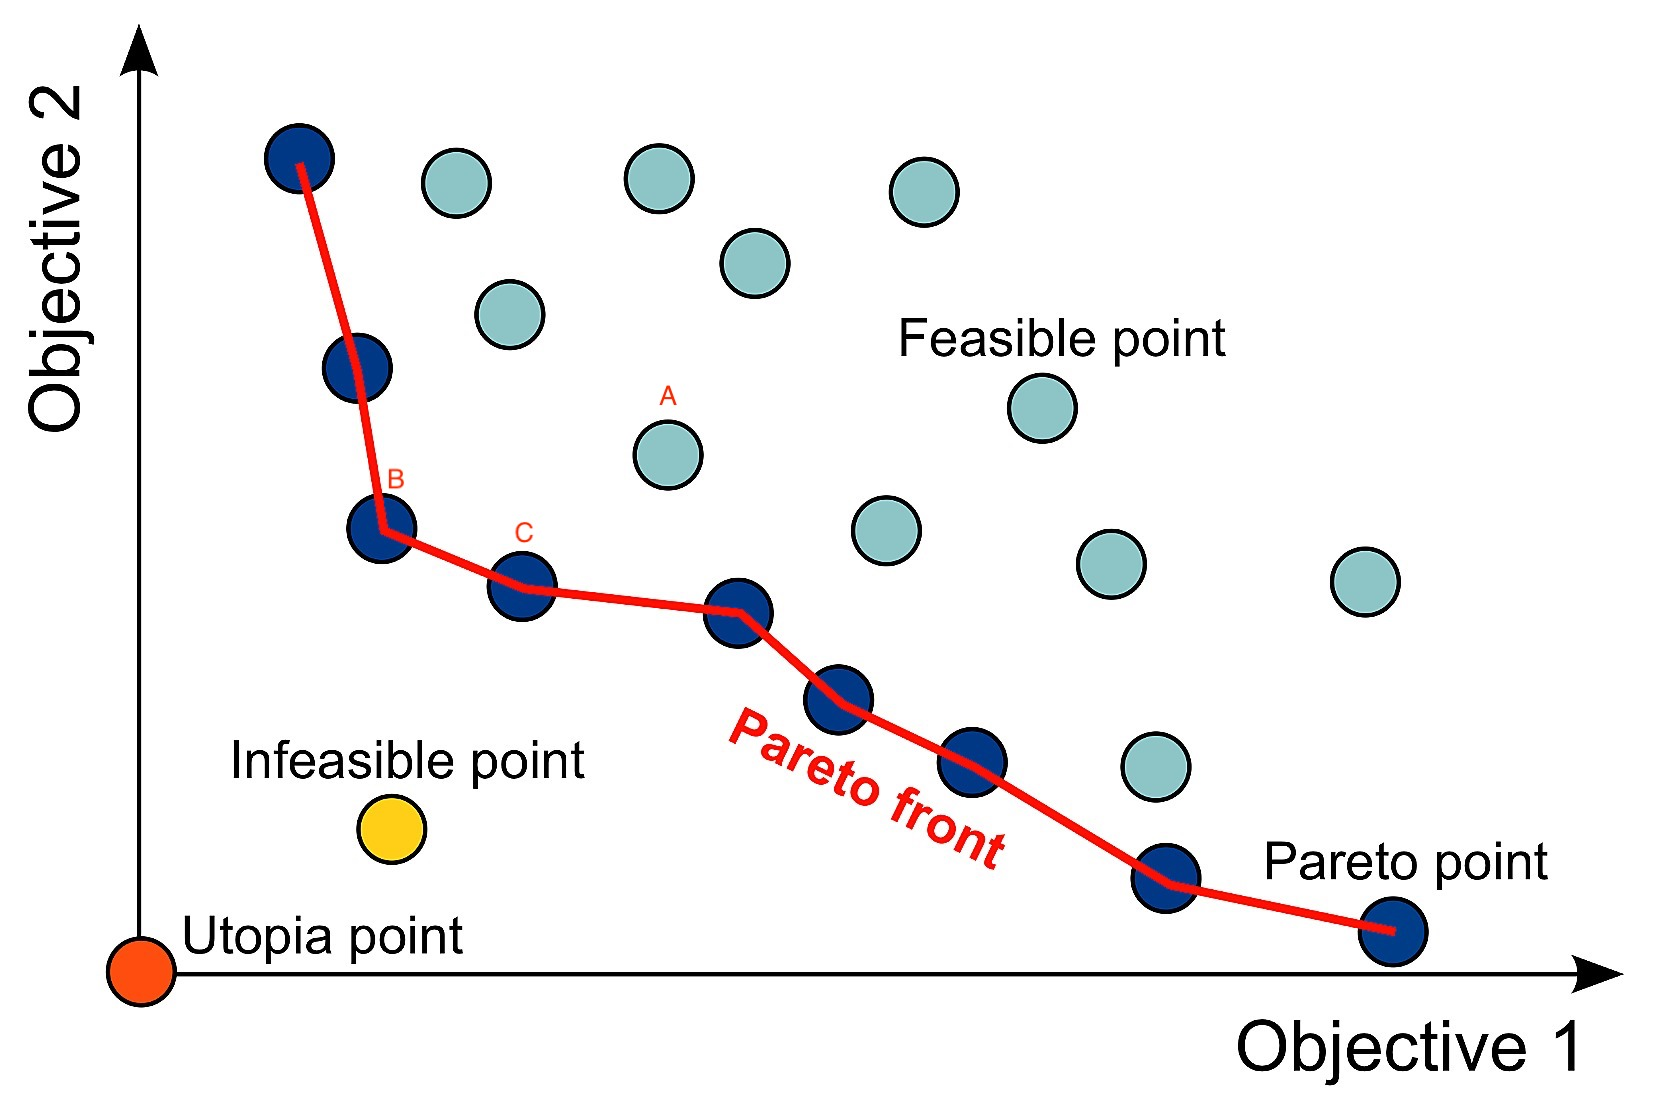
\includegraphics[width=0.66\linewidth]{img/pareto_front.JPG}
  \caption{\label{fig:paretofront}Pareto Front}
\end{figure}

Evolutionary algorithm such as the \emph{NSGA-II}\footnote{\url{https://ieeexplore.ieee.org/document/996017}} is a standard approach in solving multi-objective optimization problem. The algorithm is similar to a classical evolutionary algorithm. However the selection mechanism is different. The algorithm applies a pareto-based ranking scheme. This means that a rank is assigned to each individual based on nondominance - individuals that are not dominated by another get highest rank. Similarly as in EA, parents produce a new offspring population using genetic operators (i.e. crossover and mutation).

\begin{figure}[H]
  \centering
  \begin{subfigure}[t]{0.55\textwidth}
    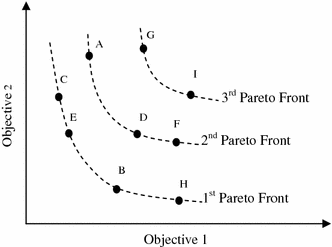
\includegraphics[width=\textwidth]{img/pareto_fronts.PNG}
    \caption{\label{fig:fronts}Pareto Fronts}
  \end{subfigure}
  \hfill
  \begin{subfigure}[t]{0.43\textwidth}
    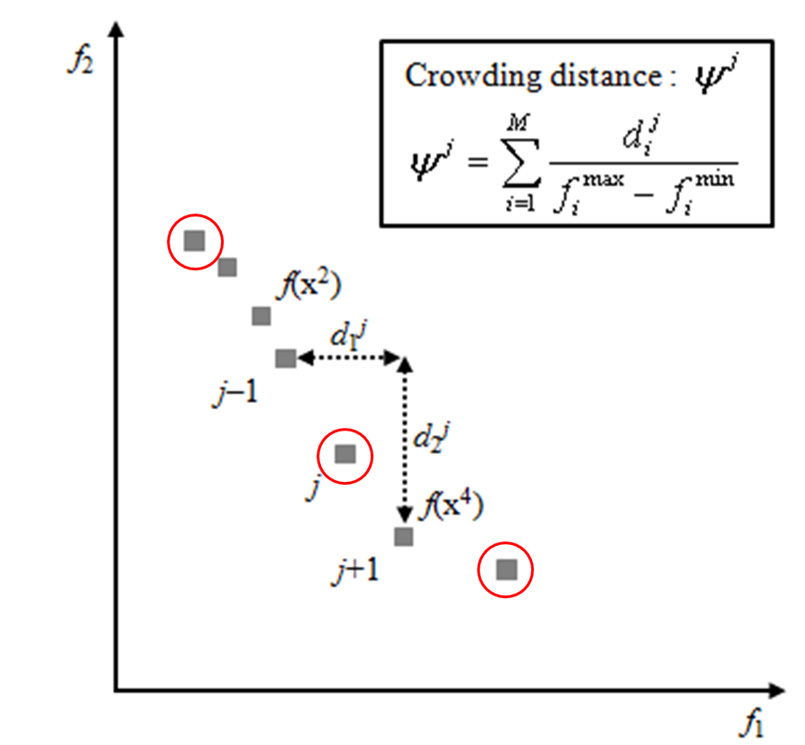
\includegraphics[width=\textwidth]{img/crowding_distance.JPEG}
    \caption{\label{fig:endings}Crowding Distance}
  \end{subfigure}
  \caption{\textit{Pareto Fronts} and \textit{Crowding Distance}.}
  \label{fig:action-ending-diagram}
\end{figure}


Parents and offsprings are combined together and are sorted into different fronts, determined by their ranking. Then a secondary sorting strategy is applied by calculating the crowding distance for each individual within their fronts. The best individuals are either in the lower fronts (assuming that the objective values are to be minimized) or in the same front with higher crowding distance. The crowding distance is calculated as the sum of the cubic distance of the objective values between the neighbouring solutions of the individual. This ensures to maintain diversity and spread of solutions - crowded solutions areas are less preferred than sparsely crowded solutions in the solution area. Next generation is created by copying the best solutions (\emph{elitism}) or the fist N individuals from the population of parents and offsprings. A more detailed flow diagram of the sorting procedure is depicted in the following figure \ref{fig:nsga}.

\begin{figure}[H]
  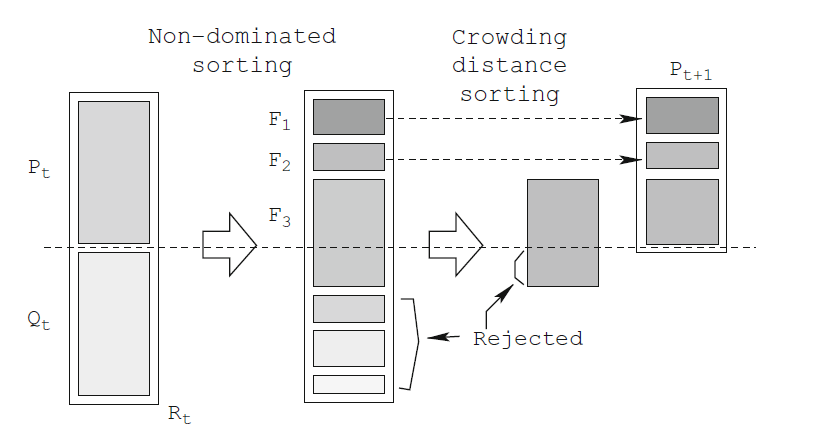
\includegraphics[width=0.66\linewidth]{img/nsga.PNG}
  \caption{\label{fig:nsga}Sorting procedure in NSGA-II}
\end{figure}

The implementation of the NSGA-II algorithm is provided by DEAP\footnote{\url{https://deap.readthedocs.io/en/master/}} evolutionary computation framework.

\subsection{NEAT}

NeuroEvolution of Augmenting Topologies \footnote{\url{http://nn.cs.utexas.edu/downloads/papers/stanley.ec02.pdf}} is a genetic algorithm for evolving both weights and topology of artificial neural networks. NEAT starts with minimal ANN structure and grows incrementally, which ensures low dimensionality of the connection weights and therefore minimizes the search space. The main traits of NEAT are \emph{genetic encoding, competing convention, speciation}.

NEAT encode networks with direct encoding schemes. The genome contains a list of \emph{connection genes} and list of \emph{nodes genes} which appears in the phenotype. Node genes represents inputs, hidden nodes, and outputs that can be connected. Whether a in-node and out-node is connected is expressed in the \emph{connection gene}. Additionally each connection gene contains a \emph{innovation} number. A genetic encoding of an individual can bee seen in figure \ref{fig:genome}.

\begin{figure}[H]
  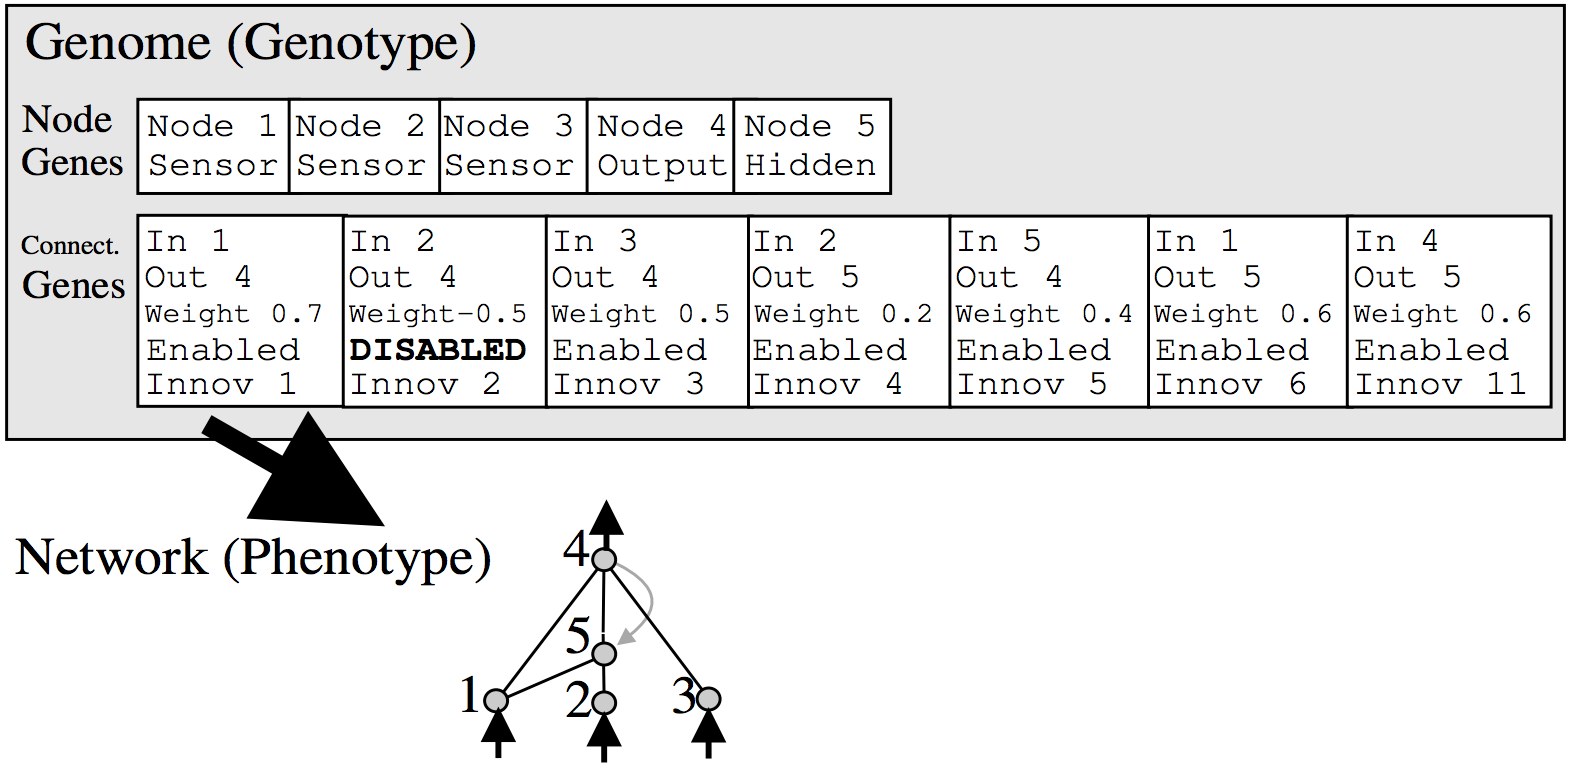
\includegraphics[width=0.66\linewidth]{img/neat_encoding.PNG}
  \caption{\label{fig:genome}Genetic encoding of individual}
\end{figure}

Mutation in NEAT can occur in three different ways. Connections weights are mutated just like in any neuroevolution, the value of the connection gene is mutated. Structural mutations are \emph{add connection and add node}. In \emph{add connection} mutation, a new connection gene is added with random weight connecting two previously unconnected nodes. Adding a new node, consists of splitting the existing connection between two nodes. The new node is added between these two previously connected nodes. The new connection leading to the new node receives the weight of 1, and the new connection leading out from the new node receives the old connection weight that was previously connecting the two nodes. The new connection of weight 1 minimize the initial affect of the mutation, this ensures that the network have time to optimize, because of \emph{speciation}. An example of this mutation can bee seen in figure\ref{fig:add_node}.

\begin{figure}[H]
  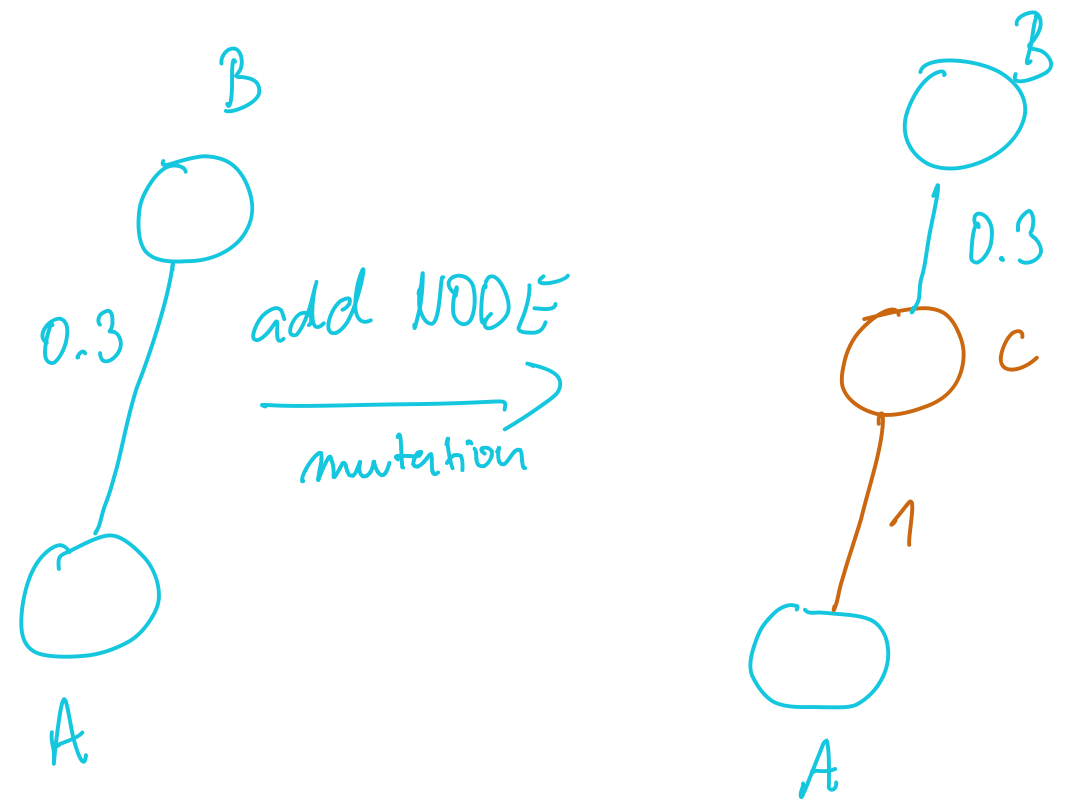
\includegraphics[width=0.56\linewidth]{img/add_node.JPEG}
  \caption{\label{fig:add_node}\emph{Add node} mutation operator in NEAT}
\end{figure}

\emph{Competing convention} is when individuals can express a solution to the same problem with different encoding. An example is depicted in figure \ref{fig:competing_convention}. The two networks compute the same function, even though their genetic encoding is different (hidden units appears in different order). This make crossover difficult, by one-point recombination of parents, both children lost crucial genetic information of their parents.

\begin{figure}[H]
  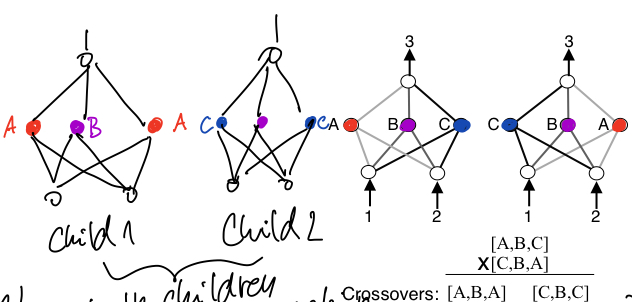
\includegraphics[width=0.56\linewidth]{img/competing_convention.JPEG}
  \caption{\label{fig:competing_convention}Competing Convention Problem}
\end{figure}

\emph{NEAT} is addressing this issues by \emph{global innovation number}, which enables genes to match up with genes of any individual in the population. More precisely, two genes with the same innovation number represents the same structure, because they are both derived from the same ancestral gene. Innovation numbers are unique and never change. Whenever two genomes mate, their offspring inherits the same innovation numbers on each gene.

When crossover is applied, the genomes are lined up with respect to the innovation number, see figure \ref{fig:crossover}. Genes that matches innovation number of both parents are called \emph{matching} gene. Genes that are not matched are called either \emph{disjoint} or \emph{excess}. During mating, \emph{matching} genes are randomly choose from either matching parent, whereas all \emph{disjoint} and \emph{excess} are included from the more fit parent.

\begin{figure}[H]
  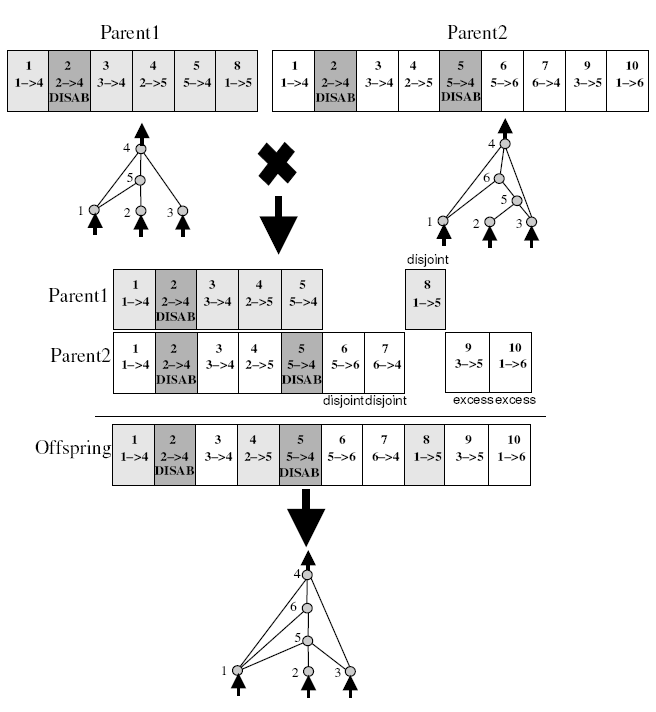
\includegraphics[width=0.5\linewidth]{img/crossover.PNG}
  \caption{\label{fig:crossover}Matching genomes innovation numbers}
\end{figure}


\emph{Speciations} in NEAT allows to divide the population into species according to topological similarities. Speciations ensures that topological innovations are protected and they have time to optimize their structure by competing within their niche. The implementation of speciation is exploited by measuring the compatibility distance according to the number of \emph{disjoint} and \emph{excess} genes between genomes. An ordered list of species is maintained. Species are represented by a random genome inside the species from previous generations. Each generation and individual is placed into the species in which the representative individual of that species is compatible with the current individual. If the individual is incompatible within any existing species, a new species is created with the individual as its representative. 


\section{Robotic Simulator}

In our experiments a set of tools is needed in order to develop, test and validate different approaches to multimodal behavior. In context of robotics, usually these tools represents robotic simulators and robotic frameworks. Robotic simulators helps to build the bridge between artificial theories and robotics. Furthermore they certify that the developed simulation can be transferred and applied to real robots. According to a survey \footnote{\url{https://ieeexplore.ieee.org/document/7041462}} by Ivaldi, Peters, the most well known robotic simulators in the community field are \emph{V-REP}\footnote{\url{https://ieeexplore.ieee.org/document/6696520}} and \emph{Gazebo}\footnote{\url{https://ieeexplore.ieee.org/abstract/document/1389727}}. Therefore, these two simulators where chosen as our robotic simulator platforms.

In Nogueira papers \footnote{\url{http://www.dca.fee.unicamp.br/~gudwin/courses/IA889/2014/IA889-02.pdf}}, these two simulators are compared in a basic robotic control logic and evolutionary robotics experiment. The authors conclusion was that V-REP is more intuitive and user-friendly simulator, and comes with various features and is less hard-ware demanding. To adhere the authors hypothesis, we tested both of the simulators.

One of the authors comparison criteria was \emph{ROS Integration}\footnote{\url{http://www.willowgarage.com/sites/default/files/icraoss09-ROS.pdf}}. \emph{ROS (Robotic Operating System)} is robotic platform framework that provides libraries and tools to develop robotic applications. The framework allows to develop large and complex robotic systems. ROS is already becoming a standard in robotics research and industry. Our experiments does not necessitate to control and manage complex robots, thus for simplicity reasons we left out \emph{ROS} and \emph{Gazebo} for the time being. However Gazebo and ROS have a strong relationship. Gazebo is the default simulator used in ROS, and have a large base of community-developed plugins and can be run as part of the ROS system. This clearly is an advantage when using both ROS and Gazebo. On the other hand V-REP doesn't have a native ROS integration, however offers a  ROS interface via plugin that comes with ROS specific features. Despite this disadvantage, V-REP offers a remote API that allows to control the simulation from external client side applications. The client side applications are available for many programming languages. Since our preferred programming language is python, which is supported by the remote API, the client side application is written in python which enables to control the simulation over the simulation variables. As pointed out by the author, Gazebo required getting and setting the position of the robot after each simulation. As we have discovered this was not needed in V-REP, because the robot was resetted to its initial position by the simulator in each simulation.

Additionally V-REP comes with numerous models that can be easily inserted in the scene. Contrary Gazebo offers limited simple geometric models that can be inserted into the scene. And these models can be only edited using external 3d-modeling tools which requires more domain knowledge about 3d modeling.

In conclusion, what we have found out is both Gazebo and V-REP do offer an API capable of controlling the simulation. Also both of them can be integrated with ROS, altought V-REP is one step behind. However, V-REP is more intuitive and user-friendly and we have experience using it from previous projects, hence, it is fair to say that we should have a better chance of implementing and validating multimodal behavior agents using V-REP rather than Gazebo.

\section{Robots}

One of the key ingredients of our experiments is the physical robot. The main role that the robot system plays in our experimental setting is a black box to be programmed in order to create a concrete physical manifestation of the evolved robot control policies. In this case the robot is not build, but rather a well functioning preassembled robot that serve as a supporting component. The primary reason for such a robot is the insufficient intellectual knowledge and experience within mechatronics and robotics. For our purposes, we focus on preexisting robotic platforms, or robotic kits, which usually comes with robot controllers and programming environments. While there are many possible robotic platforms that would fit our purposes, we mainly focused on options that are available at our hands at ITU, namely \emph{Pololu Zumo 32U4 Robot} and \emph{Thymio}.

\subsection{Zumo 32U4}

\emph{Zumo 32U4}\footnote{\url{https://www.pololu.com/category/170/zumo-32u4-robot}} is small robot that includes a built-in Arduino-compatible microcontroller, proximity sensors and line following sensors. 2 of the proximity sensors are located in front and on the sides. As it turned out the readings of the proximity sensors are really noisy and the robot has various blind spots, especially the back of the robot, since it does not have any sensors attached to it. This might lead to situations when the robot could not detect obstacles. Additionally a bluetooth module is attached to the onboard controller for wireless control of the robot and acess to sensors reading.

Unfortunately the microcontroller can't be programmed in our preferred programming language, likewise it does not expose any bindings for different programming languages. Therefore the only option is to program the microcontroller in C and create our own interface and expose that interface over serial port.

Alternative option to Zumo 32U4 robot is the Thymio that compensate certain limitation of the Zumo robot. Contrary to Zumo, Thymio has more proximity sensors and can be programmed more easily. Thymio was chosen as a robotic platform for our experiments.

\subsection{Aseba and Thymio}

\emph{Thymio}\footnote{\url{https://www.thymio.org/home-en:home}} is a small robot produced by Mobsya\footnote{\url{http://www.mobsya.org/}} for educational purposes. It has 5 proximity sensors in front, 2 proximity sensors on the back as well as 2 grounds sensors. Thymio is also equipped with temperature sensor, various buttons for interaction, visual sensors etc. Detailed overview of all the components can bee seen in figure\ref{fig:thymio}. For this experiments purposes we use the new \emph{Wireless Thymio}, which enables us to control the robot with wireless dongle.

\begin{figure}[H]
  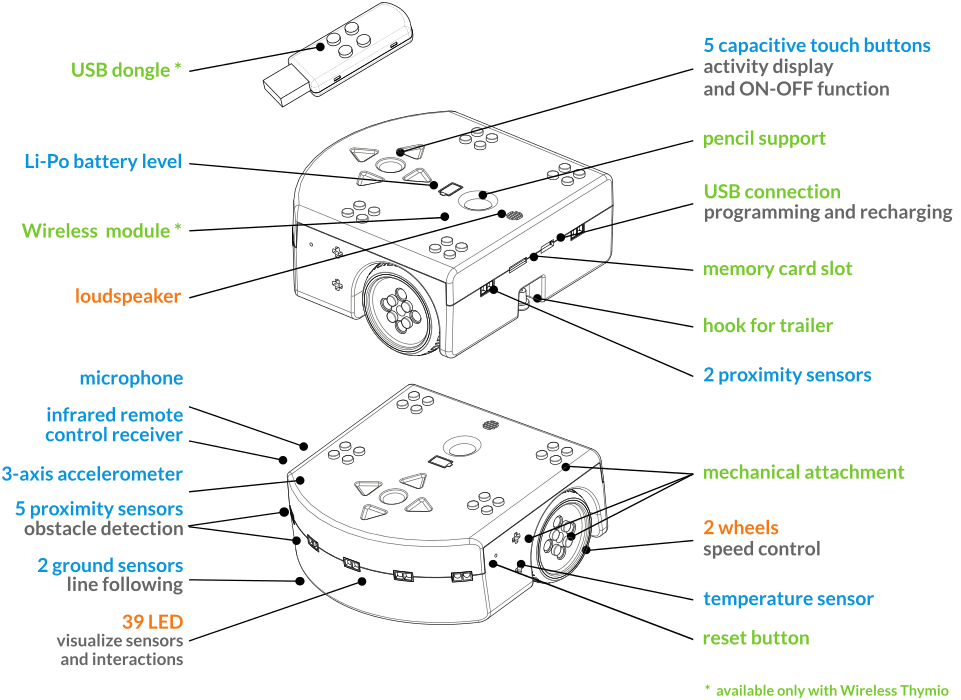
\includegraphics[width=0.6\linewidth]{img/thymio.PNG}
  \caption{\label{fig:thymio}Components of Thymio}
\end{figure}

Thymio can be programmed with \emph{Aseba}\footnote{\url{https://aseba.readthedocs.io/en/latest/about.html}}, which is set of tools that enables to program the robot within several programming environments, namely \emph{Visual, Blockly, Text, Scratch} programming. Aseba is shipped with a command-line utility tool called \emph{asebamedulla}, that allows to access an Aseba network through \emph{D-BUS}\footnote{\url{https://www.freedesktop.org/wiki/Software/dbus/}}. This enables to program Aseba-enabled devices, the Thymio robot, using third party languages, in our case Python. The \emph{Aseba Community Repository}\footnote{\url{https://github.com/aseba-community/aseba}} contains several examples how to interface with asebamedulla using D-Bus. Since our preferred language is Python, the python CLI\footnote{\url{https://github.com/aseba-community/aseba/blob/master/examples/clients/python-dbus/aseba.py}} was chosen, which is a thin wrapper around asebamedulla dbus interface. 

D-Bus is the main IPC system used in Linux: processes expose objects with a declared interfaces whose methods can be called from other processes. This is implemented by sending messages over D-Bus itself. The Aseba environment provides a D-Bus interface via the asebamedulla utility, which is in charge of transmitting to the robot hardware. The abstraction is in the form of a network of Thymio robots and processes listening on D-Bus, the so-called \emph{AsebaNetwork}. 

The goal of the Aseba D-Bus integration is not to be an alternative to any of the Aseba languages used to program the robots locally. Indeed, it is meant to provide integration with another system, on which not only the D-Bus deamon and asebamedulla are running, but also the programs utilizing the D-Bus interface, which are never transferred in any manner to the Thymio hardware. This in turn means that the robots are supposed to be continuously connected to the machine on which the Python script, in our case, is running.

The API consists ultimately in the interfaces that asebamedulla provides over D-Bus. Through this interface, we can retrieve information about the network, read and write variables, or send events.

\begin{lstlisting}[caption={\ The API that asebamedulla provides over D-Bus},language=Python,captionpos=b,label={Asebamedulla API},basicstyle=\small]
interface ch.epfl.mobots.EventFilter {
    method Void ListenEvent(UInt16 eventId)
    method Void ListenEventName(String eventName)
    method Void IgnoreEvent(UInt16 eventId)
    method Void IgnoreEventName(String eventName)
    signal Event(UInt16 id, String name, Array<SInt16> payloadData)
}

interface ch.epfl.mobots.AsebaNetwork {
    method Void LoadScripts(String fileName)
    method Array<String> GetNodesList()
    method Array<String> GetVariablesList(String nodeName)
    method Void SetVariable(String nodeName, String variableName, Array<SInt16> variableData)
    method Array<SInt16> GetVariable(String nodeName, String variableName)
    method Void SendEvent(UInt16 eventId, Array<SInt16> payloadData)
    method Void SendEventName(String eventName, Array<SInt16> payloadData)
    method ObjectPath CreateEventFilter()
}
\end{lstlisting}


The \emph{AsebaNetwork} interface allows to work with all of the nodes (robots) in the same network. There are methods to retrieve a list of the connected nodes ( \emph{GetNodesList} ) and to broadcast a global event, like \emph{SendEvent}. Global events are events that aseba nodes exchange within the aseba network. On the other hand, events that are internal to the node are called \emph{local events}. \emph{SetVariable} and \emph{GetVariable}, which write and read respectively native variables of the Aseba scripting language.

Asebamedulla expose the interface \emph{EventFilter} which allows to manage events. An application that wants to listen to events have register events with \emph{ListenEventName} or \emph{ListenEvent} be notified when an event occurs. The application can receive these events through the \emph{Event} signal, these events correspond to the global events of the Aseba language.


\section{Experiments}

Donec euismod iaculis pretium. Donec non massa elit. Phasellus sagittis magna et maximus dictum. Duis quis ullamcorper orci. Mauris interdum, elit eu tincidunt tempor, lectus mi venenatis purus, quis posuere tellus ex in magna. Phasellus tincidunt nibh eu tortor semper, et varius justo vulputate. Nullam dictum congue lacinia. Maecenas sagittis nulla quis leo fringilla viverra. Proin eget egestas nisl. Class aptent taciti sociosqu ad litora torquent per conubia nostra, per inceptos himenaeos. Pellentesque habitant morbi tristique senectus et netus et malesuada fames ac turpis egestas. Vestibulum a interdum tellus, a hendrerit ligula. Duis ut risus ut lacus maximus euismod. Integer quis justo sit amet sapien accumsan rutrum nec nec dolor. Aliquam laoreet scelerisque ante, quis hendrerit ipsum viverra tempor.


\section{Summary}

Donec euismod iaculis pretium. Donec non massa elit. Phasellus sagittis magna et maximus dictum. Duis quis ullamcorper orci. Mauris interdum, elit eu tincidunt tempor, lectus mi venenatis purus, quis posuere tellus ex in magna. Phasellus tincidunt nibh eu tortor semper, et varius justo vulputate. Nullam dictum congue lacinia. Maecenas sagittis nulla quis leo fringilla viverra. Proin eget egestas nisl. Class aptent taciti sociosqu ad litora torquent per conubia nostra, per inceptos himenaeos. Pellentesque habitant morbi tristique senectus et netus et malesuada fames ac turpis egestas. Vestibulum a interdum tellus, a hendrerit ligula. Duis ut risus ut lacus maximus euismod. Integer quis justo sit amet sapien accumsan rutrum nec nec dolor. Aliquam laoreet scelerisque ante, quis hendrerit ipsum viverra tempor.


\end{document}
